\section{Fission of Induction State}
\label{sec:fission}

\begin{figure}[t!]
\centering
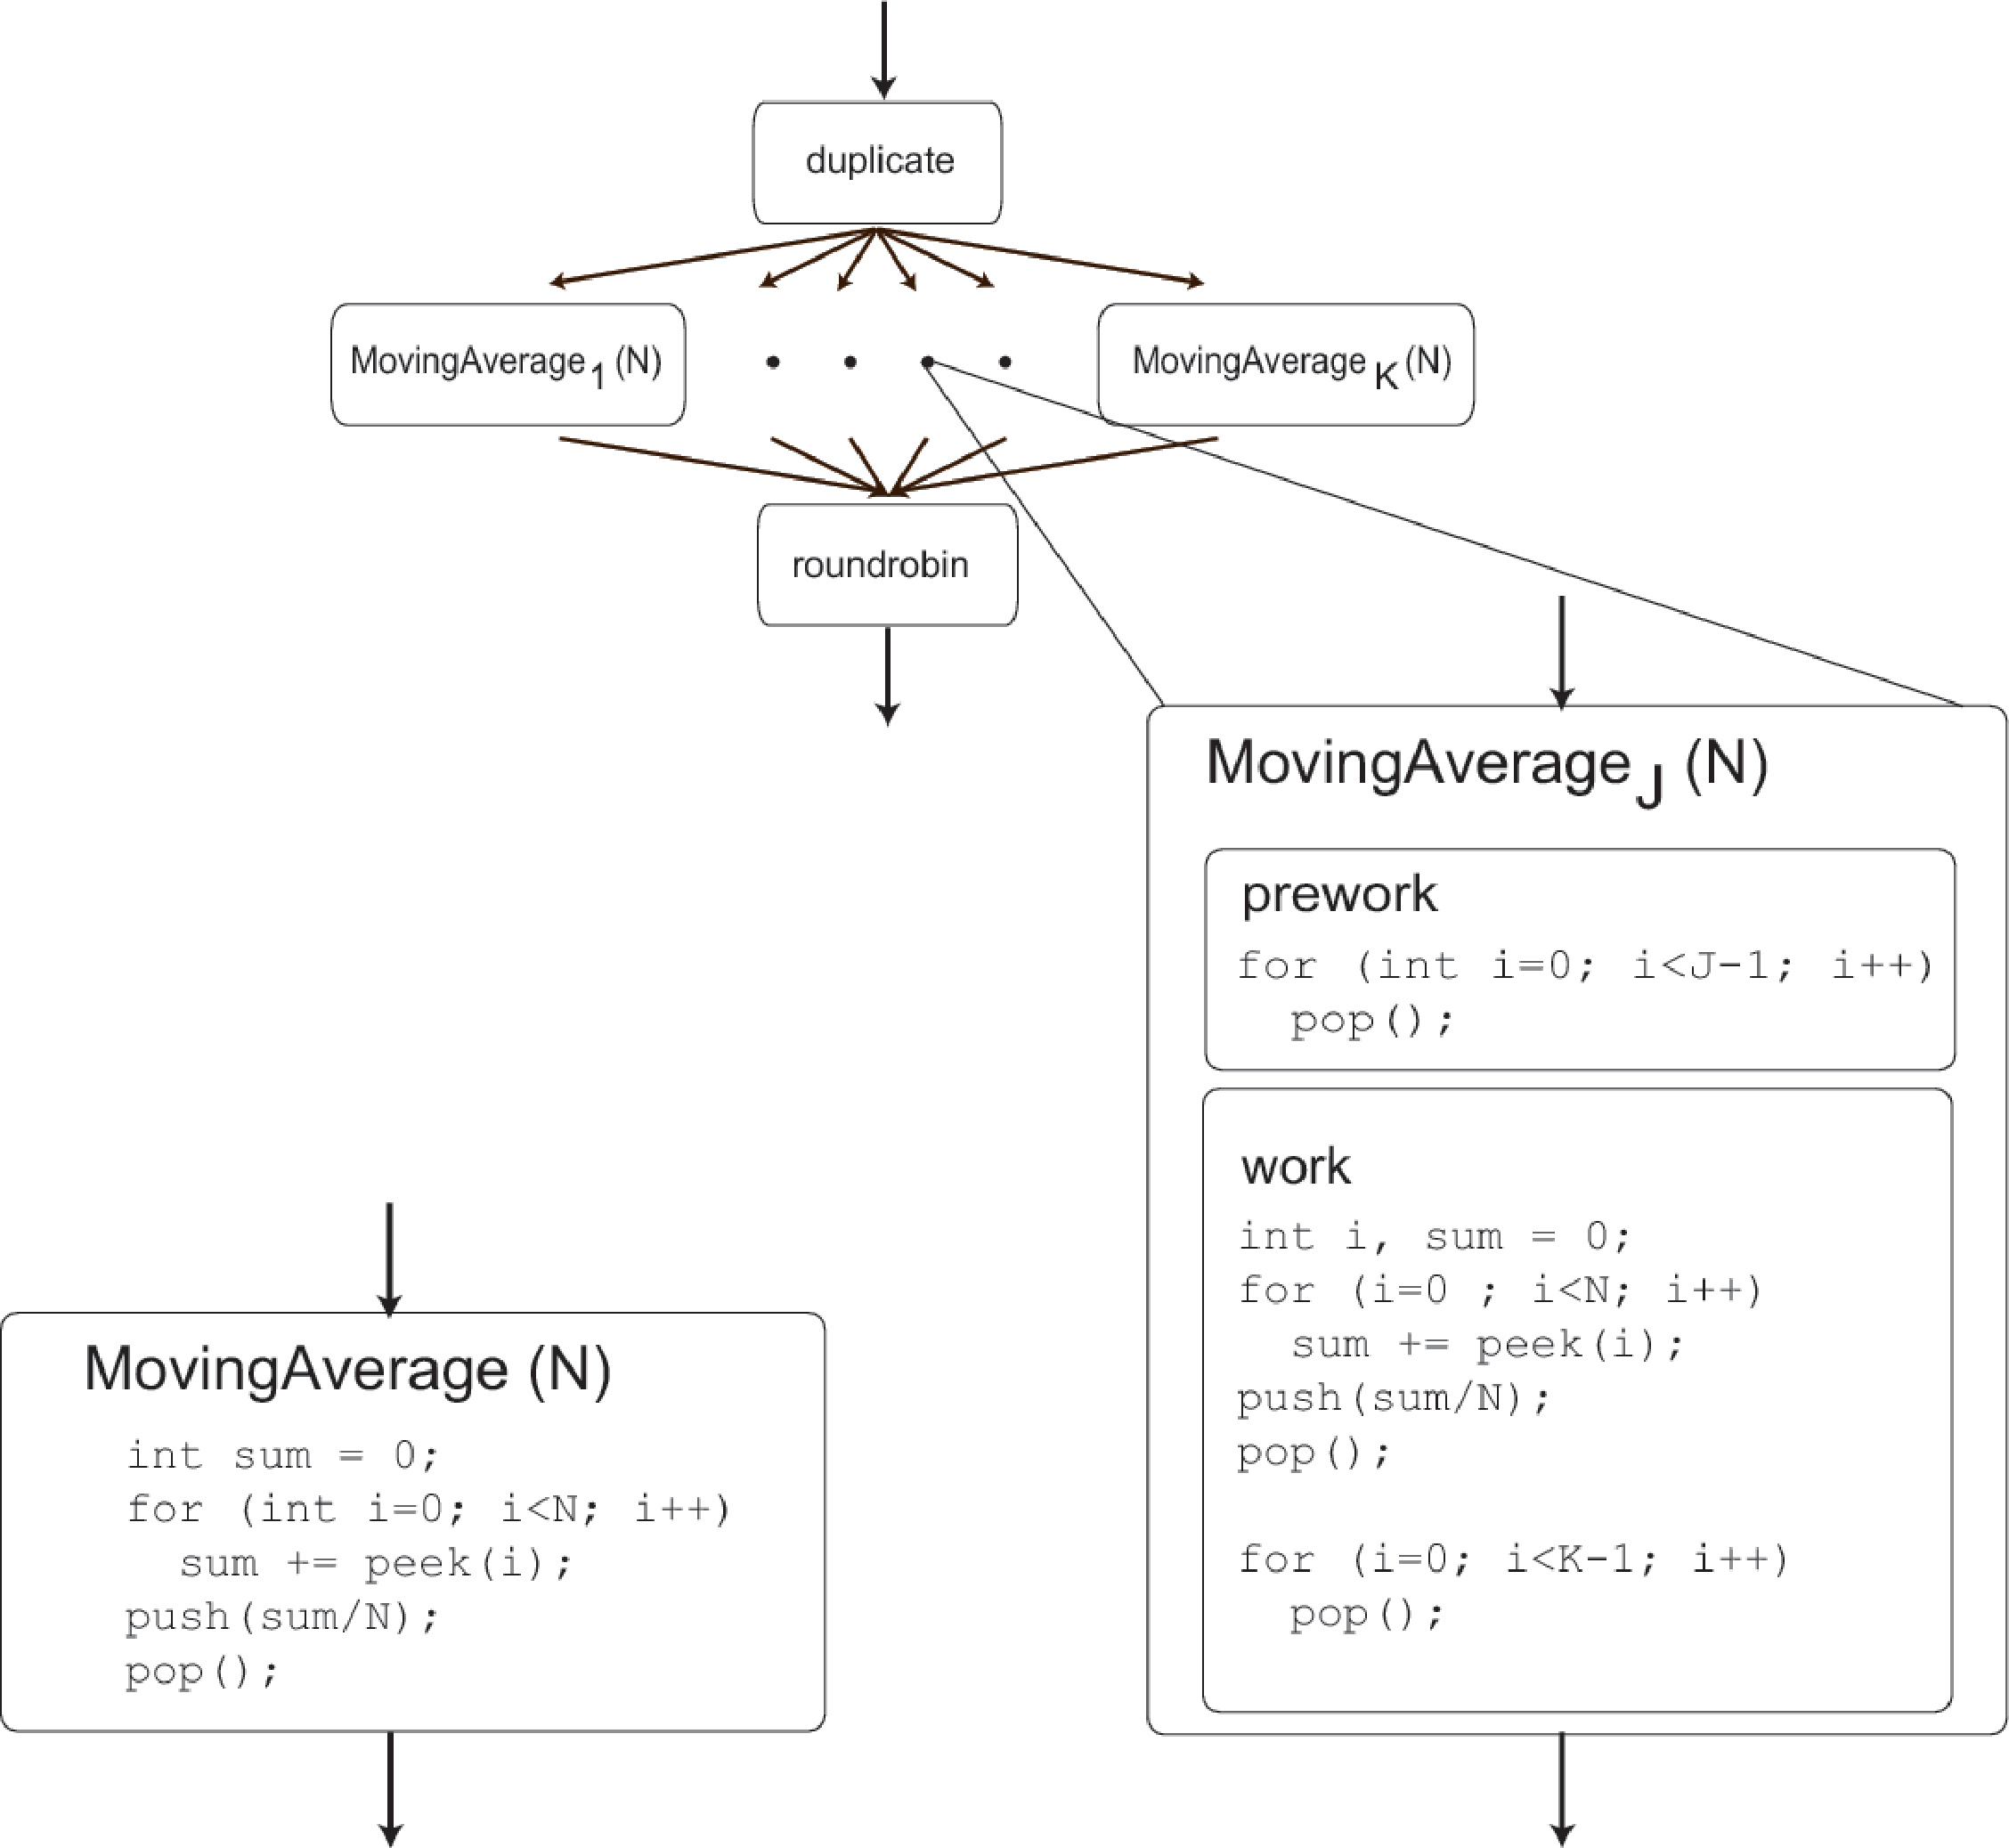
\includegraphics[width=3.4in]{figures/duplicate-fission.pdf}
\caption{Fission of a stateless filter that peeks and does not include the iteration keyword. \protect\label{fig:duplicate-fission-example}}
\end{figure}


\begin{figure*}[t!]
\centering
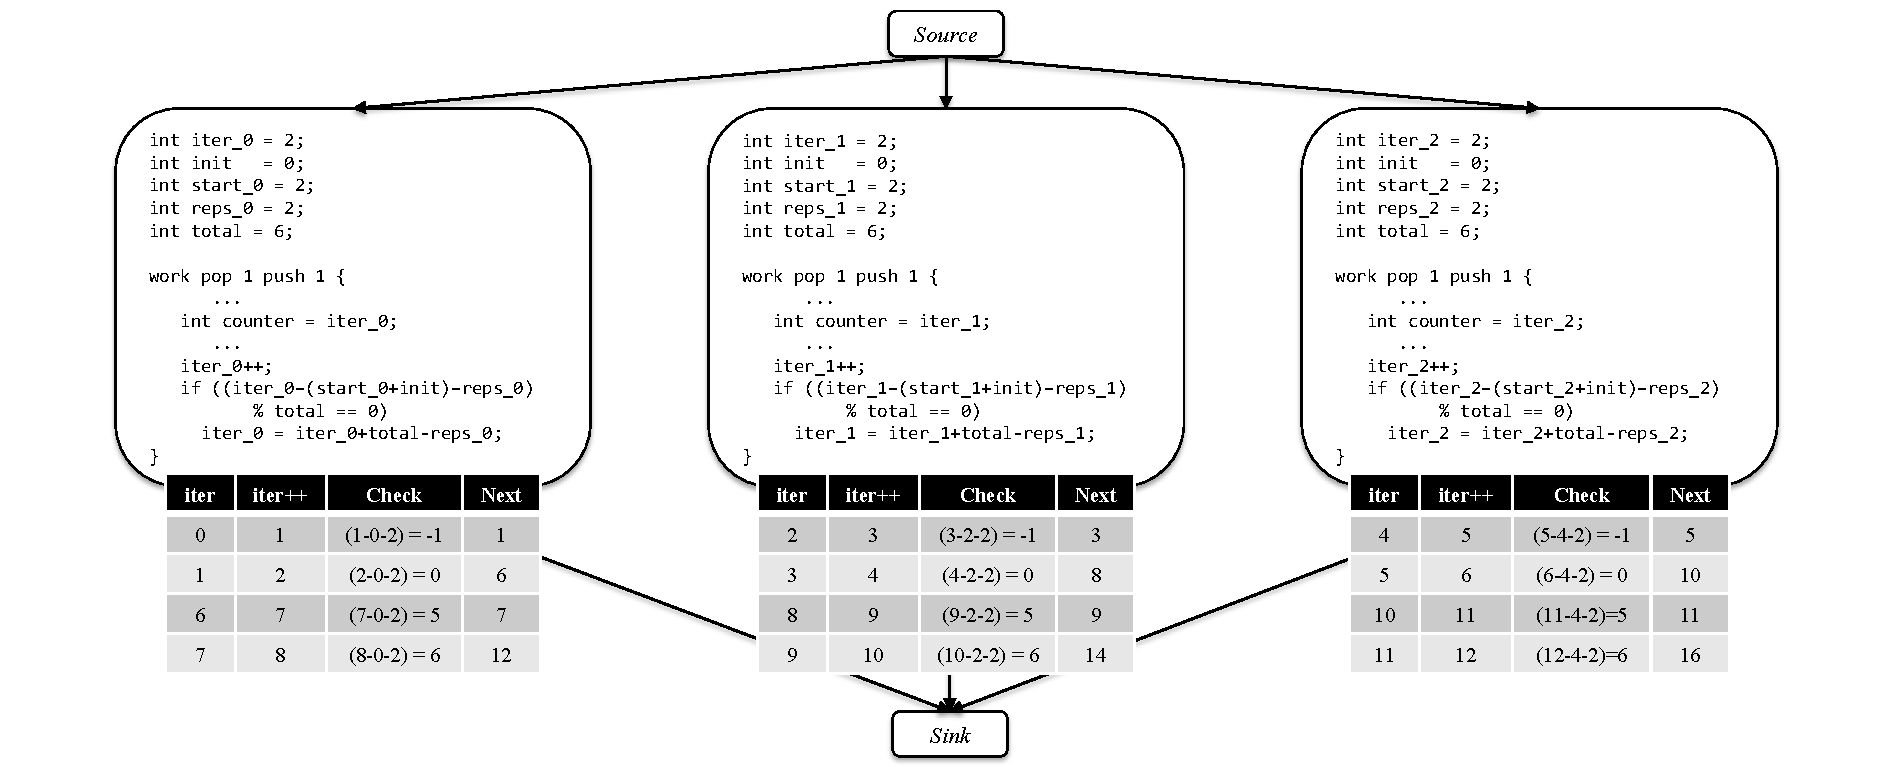
\includegraphics[width=6.5in]{figures/fission-example.pdf}
\caption{Example of an iteration filter fissed into three fission products each with multiplicity 2.  The chart indicates the values used to determine the next value of the iteration field.  
\protect\label{fig:fission-example}}
\end{figure*}

Data parallelism is added to a stream program through a transformation
known as {\it fission}. Fission is the process of duplicating a
stateless filter and wrapping these duplicates in a splitjoin so that
input data is distributed correctly and output data is collected in
correct order. The duplicated filters, known as products, can be
assigned to distinct cores, thus introducing data parallelism.

\subsection{The Original Fission Transformation}

The unmodified fission transformation is described
in~\cite{streamit-asplos}. In this section we give some background for
the transformation. The original fission transformation is applicable
only to a stateless filter, i.e., a filter that do not include a state
field to which non-constant values are assigned in the \prework or
\work functions. The simplest case for fission is when it is applied
to a filter that does not peek (i.e., the peek rate equals the pop
rate). In this case, the filter is duplicated the desired number of
ways, and placed in a round-robin splitjoin, where the weights of the
splitter are uniform and equal to the pop rate of the orignal
filter, and the weights of the joiner are uniform and equal to the
push rate of the original filter.

A more complex case is illustrated in
Figure~\ref{fig:duplicate-fission-example}. The base filter,
MovingAverage, is a peeking filter with a sliding window (the pop rate
is 1 and the peek rate is $N$). In this case the filter is placed in a
splitjoin with a duplicate spitter and a round-robin joiner. Each
individual MovingAverage$_j$ product has the \work function of the
base filter with some additional code to implement the sliding window
correctly. The duplicate splitter is introduced because of the fact
that a single input item is read by multiple filters (due to the
overlapping sliding windows between the products). All input items are
duplicated to all products, with unneeded items being decimated by
popping them at the end of the new \work function.  The \prework
function is introduced to decimate input data that is consumed by
previous products during before the first iteration.  

Providing the complete algorithm for the fission transformation is
beyond the scope of this paper, but from the example
in Figure~\ref{fig:duplicate-fission-example}, the reader can
gleam the necessary background information to understand our
modifications to the algorithm in the next section.

\subsection{Modifications to Fission Transformation}

Fission is applicable only to stateless filters, as the duplication
process does not guarantee consistent behavior if filters contain
state that changes between iterations. Because the desugared iteration
filters actually use mutable state to keep track of iteration values,
the fission process must be modified to handle iteration values. If a
filter includes only state in the form of the {\it iter} field
introduced by the desugaring process (see \S\ref{sec:desugar}), then
it is considered a candidate for the modified fission process
described in this section.

The code additions described below are applied to the fission products
after the original fission transformation algorithm introduces the
splitjoin structure and (for peeking filters) makes it changes to the
\work and \prework functions.

Let $F$ be the stateless filter that will be fissed. Assume the
fission process yields $N$ fissed products. Accordingly, this yields
the fissed products $F_0$, $F_1$, ... , $F_i$, ... , $F_{N-1}$. The
notation $F_{i}$ represents the $(i+1)$th fissed product of filter
$F$.

The fission process now modifies the fission products by adding the
following values as fields to the products:
\begin{itemize}
    \item \texttt{init}: the multiplicity of the initialization schedule.  This value is determined for $F$ and is constant for all fissed products.
    \item $\texttt{reps}_i$: how often the \work function of the product $F_i$ is
      invoked between rounds.
    \item $\texttt{start}_i$: the value of the induction variable each product $F_i$ starts with, less the initialization multiplicity.  Alternatively, $\sum_{j=0}^{i-1}{\tt reps}_j$ of all fission products preceding the current product.
    \item \texttt{total}: the periodic multiplicity of $F$.  Alternatively $\sum_{j=0}^{N-1}{\tt reps}_j$. This value is the same for all fissed products.
\end{itemize}
As described in~\S\ref{sec:streamit}, initialization execution is required for peeking filters to ensure every firing of the periodic steady-state schedule maintains the same number of leftover items on the channel.  This initialization execution of the original filter is transferred entirely to the first fission product.  However, all fission products must take the multiplicity of the initialization schedule into account in their calculations as the multiplicity is adjusted upwards by this value.

Accordingly, the fission product $F_i$ should start each round with iteration values of
\begin{eqnarray*}
\texttt{total}*\texttt{k} + (\texttt{start}_i + \texttt{init})
\end{eqnarray*}
and range up to the value
\begin{eqnarray*}
\texttt{total}*\texttt{k} + (\texttt{start}_i + \texttt{init}) + \texttt{reps}_i - 1
\end{eqnarray*}
where \texttt{k} is a nonnegative integer indicating how many rounds have
been run in the span of the program.  

At the end of each fission product's \work, a check must be made to
see if it is necessary to increment the induction variable to the next
round of values.  This will prevent certain fissed products from
making calls with duplicate iteration values.  This check is done
after the field incrementing statement.

\begin{eqnarray*}
(\texttt{iter}_{i,k} - (\texttt{start}_i + \texttt{init}) - \texttt{reps}_i) \% \texttt{total} &==& 0
\end{eqnarray*}

This is consistent with the maximum value per round as
indicated above.  Only when we reach this maximum value does subtracting 
$\texttt{start}_i$, \texttt{init}, and $\texttt{reps}_i$ from $\texttt{iter}_i$ leave a value divisible by
\texttt{total}.

Once the fissed product's iteration value has reached
this value, it must be set to:
\begin{eqnarray*}
\texttt{iter}_{i,k+1} &=& \texttt{iter}_{i,k} + (\texttt{total} - \texttt{reps}_i) \\
&=& \texttt{total}*\texttt{k} + (\texttt{start}_i + \texttt{init}) + \texttt{reps}_i \\
&&  \ \ +\ (\texttt{total} - \texttt{reps}_i) \\
&=& \texttt{total}*(\texttt{k+1}) + (\texttt{start}_i + \texttt{init})
\end{eqnarray*}
which is the starting iteration value of the next round, as defined.

Figure~\ref{fig:fission-example} shows the filter from Figure~\ref{fig:desugar} fissed into three fission products, each with multiplicity 2.  The accompanying charts for each fissed product are as follows:
\begin{itemize}
\item{\tt iter} indicates the value of the {\tt iter} field at the start of the filter invocation.  
\item{\tt iter++} indicates the value of the {\tt iter} field incremented by 1 (which is the value {\tt iter} takes prior to the check.  
\item{\tt check} indicates the value of $(\texttt{iter}_{i,k} - (\texttt{start}_i + \texttt{init}) - \texttt{reps}_i)$, which must be divisible by {\tt total} in order to advance to the next round.  
\item{\tt next} indicates the value {\tt iter} will take at the next invocation of the fissed product.
\end{itemize}
Note that the value of \texttt{iter} jumps to the next round of values with multiplicity 2, as expected.

\subsubsection{Accounting for Steady-state Schedule Modification}
\label{sec:ssmod}

The code additions described above are dependent on specific values
for the initialization and steady-state multiplicities of the fission
products. If any multiplicities change, then the values used in the
generated code must be updated. The initialization schedule is not
modified once it is calculated, but certain passes in the StreamIt
compiler may modify the steady-state schedule after fission,
increasing the multiplicity of the fission products.  In this section
we demonstrate how passes that run after fission and seek to
modify the steady-state must update the generated fields.

Increasing the steady-state scales the $\texttt{reps}_i$ field for all
products. $\texttt{start}_i$ and $\texttt{total}$ are dependent on
$\texttt{reps}_i$ and must be scaled accordingly. Assume a pass
increases the steady-state multiplicity of our filter to $m$. The
generated fields for product $F_i$ are updated as follows:

\begin{itemize}
    \item \texttt{init}: unchanged because the initialization schedule
      in unmodified when the steady-state is increased.
    \item $\texttt{reps}_i = \texttt{reps}_i * m $
    \item $\texttt{start}_i = \texttt{start}_i * m$
    \item $\texttt{total} = \texttt{total} * m$
\end{itemize}

After we increase the multiplicities, the values of the four fields
introduced by the transformation are consistent, i.e., the iteration
values will be correctly redistributed to account for the modification
to the steady-state multiplicities.  

% More specifically, after the increase the steady-state by $m$, the
% fission product $F_i$ starts round $k$ with an iteration value of

% \begin{eqnarray*}
% (\texttt{total}*\texttt{k}*m) + (\texttt{start}_i*m + \texttt{init})
% \end{eqnarray*}

% The filter executes $\texttt{reps}_i$*$m$ iterations, thus the final
% value for $\texttt{iter}_{i,k}$ is 

% \begin{eqnarray*}
% (\texttt{total}*\texttt{k}*m) + (\texttt{start}_i*m + \texttt{init}) + (\texttt{reps}_i*m) - 1
% \end{eqnarray*}

% Between rounds, iteration values must be incremented by the actual
% total number of repetitions that occur.  All fission products perform
% a total of $\sum(\texttt{reps}_{i}*m)$ repetitions which is simply
% \texttt{total}*$m$.  Thus, the updating step will still hold:

% \begin{eqnarray*}
% \texttt{iter}_{i,k+1} &=& \texttt{iter}_{i,k} + (\texttt{total}*m - \texttt{reps}_i*m) \\
% &=& \texttt{total}*\texttt{k}*m + (\texttt{start}_i*m + \texttt{init}) + \texttt{reps}_i*m \\
% &&  \ \ +\ (\texttt{total}*m - \texttt{reps}_i*m) \\
% &=& \texttt{total}*(\texttt{k+1})*m + (\texttt{start}_i*m + \texttt{init})
% \end{eqnarray*}

% \todo{put something here that wraps up the proof}

